

%----------------------------------------------------------------------------------------
%	PACKAGES AND OTHER DOCUMENT CONFIGURATIONS
%----------------------------------------------------------------------------------------

\documentclass[twoside,twocolumn]{article}

\usepackage{blindtext} % Package to generate dummy text throughout this template 
\usepackage{graphicx}
\usepackage{listings}
\usepackage{color}
\usepackage{float}
\usepackage{wrapfig}
\usepackage[sc]{mathpazo} % Use the Palatino font
\usepackage[T1]{fontenc} % Use 8-bit encoding that has 256 glyphs
\linespread{1.05} % Line spacing - Palatino needs more space between lines
\usepackage{microtype} % Slightly tweak font spacing for aesthetics

\usepackage[english]{babel} % Language hyphenation and typographical rules

\usepackage[hmarginratio=1:1,top=32mm,columnsep=20pt]{geometry} % Document margins
\usepackage[hang, small,labelfont=bf,up,textfont=it,up]{caption} % Custom captions under/above floats in tables or figures
\usepackage{booktabs} % Horizontal rules in tables

\usepackage{lettrine} % The lettrine is the first enlarged letter at the beginning of the text

\usepackage{enumitem} % Customized lists
\setlist[itemize]{noitemsep} % Make itemize lists more compact

\usepackage{abstract} % Allows abstract customization
\renewcommand{\abstractnamefont}{\normalfont\bfseries} % Set the "Abstract" text to bold
\renewcommand{\abstracttextfont}{\normalfont\small\itshape} % Set the abstract itself to small italic text

\usepackage{titlesec} % Allows customization of titles
\renewcommand\thesection{\Roman{section}} % Roman numerals for the sections
\renewcommand\thesubsection{\roman{subsection}} % roman numerals for subsections
\titleformat{\section}[block]{\large\scshape\centering}{\thesection.}{1em}{} % Change the look of the section titles
\titleformat{\subsection}[block]{\large}{\thesubsection.}{1em}{} % Change the look of the section titles

\usepackage{fancyhdr} % Headers and footers
\pagestyle{fancy} % All pages have headers and footers
\fancyhead{} % Blank out the default header
\fancyfoot{} % Blank out the default footer
\fancyfoot[RO,LE]{\thepage} % Custom footer text

\usepackage{titling} % Customizing the title section

\usepackage{hyperref} % For hyperlinks in the PDF





\setlength{\droptitle}{-4\baselineskip} % Move the title up

\pretitle{\begin{center}\Huge\bfseries}
\posttitle{\end{center}} % Article title closing formatting
\title{Product Recommendational System} % Article title
\author{%
\textsc{Alexandr Mirzak}\thanks{Thanks to YOU for reading this!} \\[1ex] % Your name
\normalsize NATIONAL RESEARCH UNIVERSITY HIGHER
SCHOOL OF ECONOMICS
 \\ % Your institution
\normalsize \href{mailto:asmirzak@edu.hse.ru}{asmirzak@edu.hse.ru}
}
\date{\today} 
\renewcommand{\maketitlehookd}{%
\begin{abstract}
\noindent Each day more and more products are being manufactured and typical
buyer is often struggling with a hard task of choosing the one he needs
as manually browsing through all of the is not an easy option. So,
recommendational systems based on different algorithms are taking
place. In this work I created programing interface, which serves as a
way for web services to communicate with each other, in this interface
a simple, yet scalable recommendational system was developed, which
can be used as a base for an online shop programming interface, once
connected to its product database.

\end{abstract}
}


\definecolor{dkgreen}{rgb}{0,0.6,0}
\definecolor{gray}{rgb}{0.5,0.5,0.5}
\definecolor{mauve}{rgb}{0.58,0,0.82}

\lstset{frame=tb,
  language=Python,
  aboveskip=3mm,
  belowskip=3mm,
  showstringspaces=false,
  columns=flexible,
  basicstyle={\small\ttfamily},
  numbers=none,
  numberstyle=\tiny\color{gray},
  keywordstyle=\color{blue},
  commentstyle=\color{dkgreen},
  stringstyle=\color{mauve},
  breaklines=true,
  breakatwhitespace=true,
  tabsize=3
}




\begin{document}

\Large\tableofcontents


% Print the title
\maketitle

%----------------------------------------------------------------------------------------
%	ARTICLE CONTENTS
%----------------------------------------------------------------------------------------


\section{Introduction}
\subsection{Main result}

\lettrine[nindent=0em,lines=3]{T}  he main result for this project is an attempt to create a web application
program interface that allows a user to browse through products and run
recommendation programs based on the user’s searches to improve the
probability of buying certain product by recommending similar ones
lying in the same cluster.

\subsection{instruments}
\begin{enumerate}
    \item FastAPI
    \item Python, Anaconda, Jupyter Notebook
    \item Numpy, Pandas, Matplotlib, Sklearn, SQLalchemy, Pydantic
    \item Raw unfiltered data of Walmart products listings
    \item PowerPoint
    \item Flourish.studio

\end{enumerate}

%------------------------------------------------

\section{About}

\subsection{Reviewing abstracts and analogues}

There are a lot of approaches to recommendations for users (Collaborative
filtering, Content-based filtering, Session-based recommender systems, Multicriteria recommender systems, etc.) 

However all of these approaches are hard to
implement and require lots of resources, so the clustering approach with k-Means clustering method was selected

\begin{center}
\textbf{Algorithm of KMeans}
\end{center}

The Kmeans algorithm is an iterative technique that attempts to split a dataset into
K separate non-overlapping subgroups (clusters), each of which contains only one
data point, the number of groups is completely predetermined by user, so it is
crucial to choose the optimal number of groups. It attempts to make intra-cluster
data points as comparable as possible while maintaining clusters as distinct (far) as
possible. It distributes data points to clusters in such a way that the sum of the
squared distances between them and the cluster's centroid (the mean of all data
points in that cluster) is as small as possible.
(\begin{math} 
\underset{\mathbf{S}}{\arg \min } \sum_{i=1}^{k} \sum_{\mathbf{x} \in S_{i}}\left\|\mathbf{x}-\boldsymbol{\mu}_{i}\right\|^{2}=\underset{\mathbf{S}}{\arg \min } \sum_{i=1}^{k}\left|S_{i}\right| \operatorname{Var} S_{i}
\end{math})


Within clusters, the less variation
there is, the more homogenous or similar the data points are.\cite{hartigan1979algorithm} This method of
clustering is relatively good scaling to bigger datasets, the shapes and sizes of
clusters may be of different sizes, allowing for more flexibility. However, this
method has some disadvantages, which are needed to be aware of. The main of
them are: Relatively bad clustering for outliers, as they may vary sum of squares
significantly and shift the centroids, scaling with the number of dimensions is also
a major problem of this method, thus the number of dimensions must be reduced.

The more precise description of the algorithms work is as follows: 
Given an initial set of $k$ means $m_{1}^{(1)}, \ldots, m_{k}^{(1)}$ (see below), the algorithm proceeds by alternating between two steps: 

\textbf{Assignment step}: Assign each observation to the cluster with the nearest mean: that with the least squared Euclidean (istance. this means partitioning the observations according to the Voronoi diagram generated by the means.)
\begin{equation}
\resizebox{.5\textwidth}{!}{S_{i}^{(t)}=\left\{x_{p}:\left\|x_{p}-m_{i}^{(t)}\right\|^{2} \leq\left\|x_{p}-m_{j}^{(t)}\right\|^{2}\right\}}
\end{equation}
where each $x_{p}$ is assigned to exactly one $S^{(t)}$, even if it could be assigned to two or more of them.

\textbf{Update step}: Recalculate means (centroids) for observations assigned to each cluster.

\begin{equation}
m_{i}^{(t+1)}=\frac{1}{\left|S_{i}^{(t)}\right|} \sum_{x_{j} \in S_{i}^{(t)}} x_{j}
\end{equation}
The algorithm has converged when the assignments no longer change. The algorithm is not guaranteed to find the optimum.



\subsection{Project tasks and objectives}

The projects tasks were as follows:

\begin{itemize}

\item Create an API that can be used to obtain information about
products
\item Create a database to store information about all operations and
products
\item Implement user authorization for operations
\item Develop a clusterization system for product

\end{itemize}

\textbf{Technical requirements are:}

\begin{itemize}
    \item Authorization
    \begin{enumerate}
        \item User authentication
        \item password hashing
        \item token validation
    \end{enumerate}
    \item Getting a product information by its ID
    \item Searching by a word 
    \begin{enumerate}
        \item implementing Full-Text-search
        \item text vectorization
        \item some other strange requirement
    \end{enumerate}
    \item function starting the recommendation algorithm
\end{itemize}



%------------------------------------------------

\section{List of methods, algorithms and models}

\subsection{Overall architecture review}

\begin{wrapfigure}{r}{0.16\textwidth}
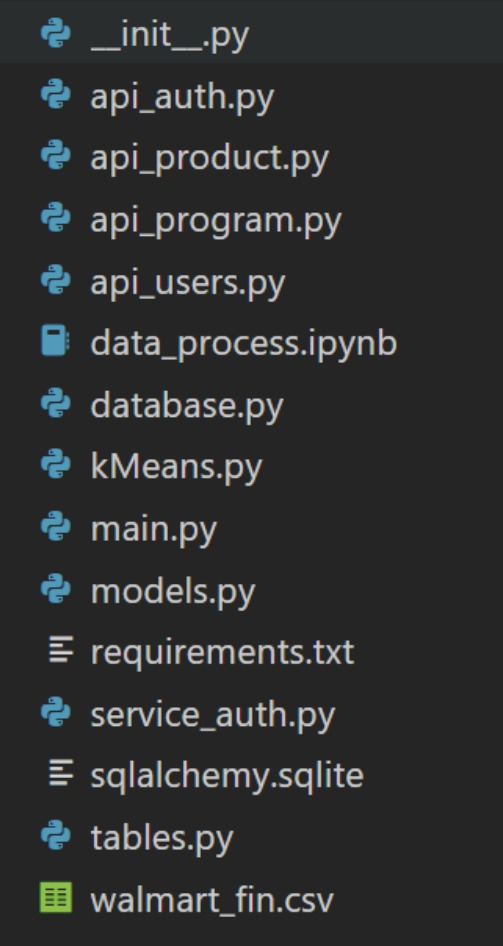
\includegraphics[width=0.22\textwidth]{images/methods.jpg}
\caption{Modules overview}
\label{fig:methods}
\end{wrapfigure}
The application has been divided into
several modules \ref{fig:methods} for a clear and
precise separation of logic as well as
ease of development. API modules
stand for describing and
implementing path operations,
dataprocess stands for
preprocessing raw data from Walmart
listings. database includes all
necessary operations for creating
dataset and pushing data into it.
kMeans includes the program for
user to run. Models consist of all the
necessary models for data to be sent
and received correctly. serviceauth
consist of all the necessary “service”
functions for authorization and tables
stand for multiple tables inside the
database that reveal its structure.
These modules will be further
explained below.

\subsection{Creating DataBase}

To store information about products, users, etc., you will need a table
system, in other words, a database. I used SQLAlchemy plugin because
of its unique approach to the database itself: it considers the database to
be a relational algebra engine, not just a collection of tables. The
following tables were needed to fully achieve the tasks set: products,
users, experiments and recommendations.

Here is a structure of a database:

\begin{table}[h]
\centering
\caption{Database stucture}
\begin{tabular}{lll}
\centering
Products & Categories & Experiments  \\
\hline \hline 
1.P_id & 1.C_id & 1.U_id & 1.Exp_id & 1.Exp_id \\
\hline 
2.Title & 2.Title & 2.Username  \\
\hline
3.Description & 3.Description & 3.Email  \\
\hline
4.Category & & 4.P_hash  \\
\hline
\end{tabular}
\end{table}

The ‘Category’ from products is a Foreign Key to the Categories.Title,
which means that only products of existing categories can be present in
the table. In the Experiments table two columns represent start and end
of the work of the recommendation algorithm. After the end of the work,
information about the obtained clusterization is put into the
recommendations table. 

After creating these tables I created the function that opens session to
enable data read and write inside the path operation functions and closes
it when the path operation function stops:


\begin{lstlisting}
$def new_session() -> Session:
 session = Session()
 try :
  yield session
 finally:
  session.close()$

\end{lstlisting}

\subsection{Setting up API}

I used FastAPI library to create an instance of FastAPI() class, which is
the app itself. Then I added the router which allowed me to add default
prefix to each of the “ApiX” folders (For example, path operations on
ApiProduct.py module now all start with prefix ‘/products’), which
allows for more clean way of representing paths. 

\begin{lstlisting}

router = APIRouter( prefix='/products')
\end{lstlisting}


\subsection{User Authorization and authentication}

Since this program can be used by several users, it is necessary to delimit access
for more accurate and secure use. For this purpose, the possibility of authorization
and authentication has been created, so the user can receive product
recommendations based on their search.

A simple approach to storing passwords is to create a table in our
database that maps a username with a password. When a user logs in, the
server receives an authentication request with a payload containing the
username and password. It is incredibly dangerous to store passwords as
a plain text in a table. A much safer way is to hash the password when
the user signs up, then store the hashed password and for login compare
not the password, but the hashed version of it. 

For this purpose, a new class AuthService was created, which allows for
registration of new users as well as authentication existing ones and
authorizing them. It uses JWT (JSON Web Token)\cite{jones2015json} as a response model
for signing up and signing in, which features a signature that can be
validated using the “secret key” – a predetermined string.\cite{bhanot2015review} This is an
example of decoding \ref{fig:dec} a token 

To authorize user for each operation that requires it (running a program, getting
information about a product or finding similar ones) I wrote a function
GetCurrentUser, which validates the received token and gives a ModelUser as
output and denies access in the case when the user in not logged in

\begin{figure}[h]
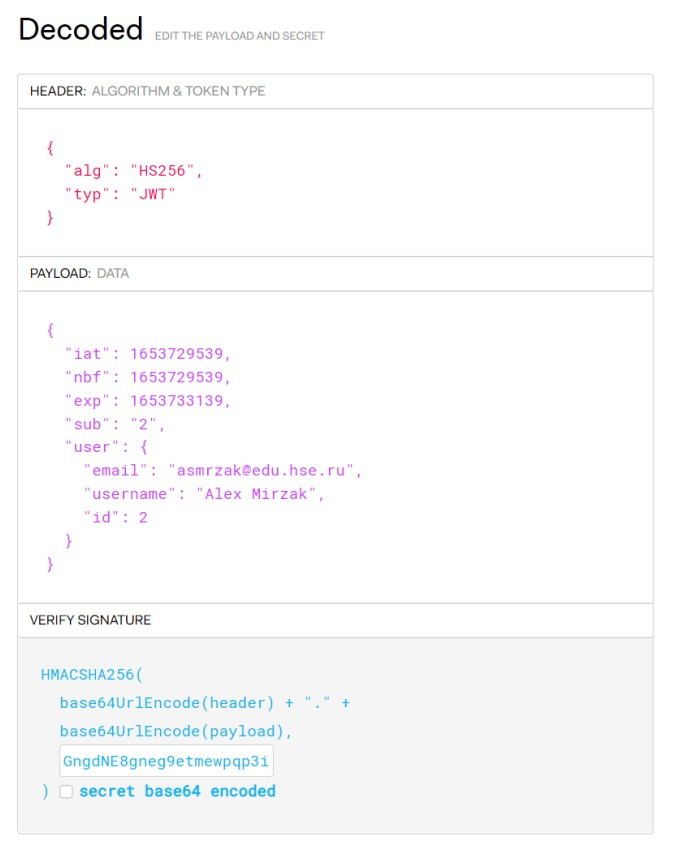
\includegraphics[width=1\linewidth, height=6cm]{images/decoded.jpg} 
\caption{decoded token}
\label{fig:dec}
\end{figure}


\begin{figure}[h]
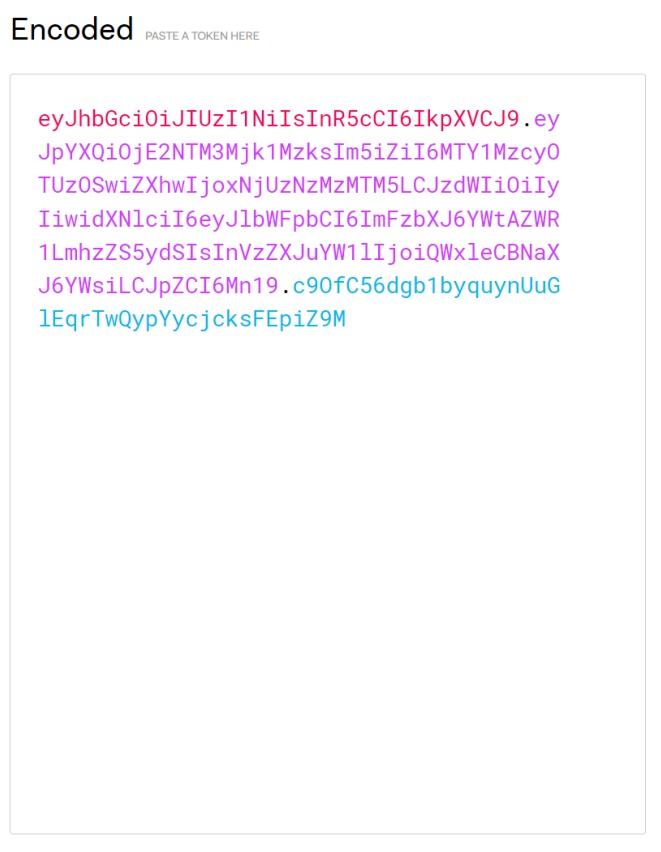
\includegraphics[width=1\linewidth, height=6cm]{images/encoded.jpg}
\caption{encoded token}
\label{fig:enc}
\end{figure}

\subsection{K-Means Elbow Method}

The k-Means algorithm is an unsupervised machine learning algorithm that divides
data into k clusters. The number of clusters is set by the user, and the algorithm
will attempt to group the data even if this number is not optimal in this
circumstance.
When the centers are plotted and the pattern seems to be an inverted triangle,
shaped like an elbow, the value at “breaking point” is the most optimal, as after it
no considerable reduction in sum of squared distances happen. After fitting model
in a range of clusters I obtained this graph \ref{fig:elb}


\begin{figure}[h]
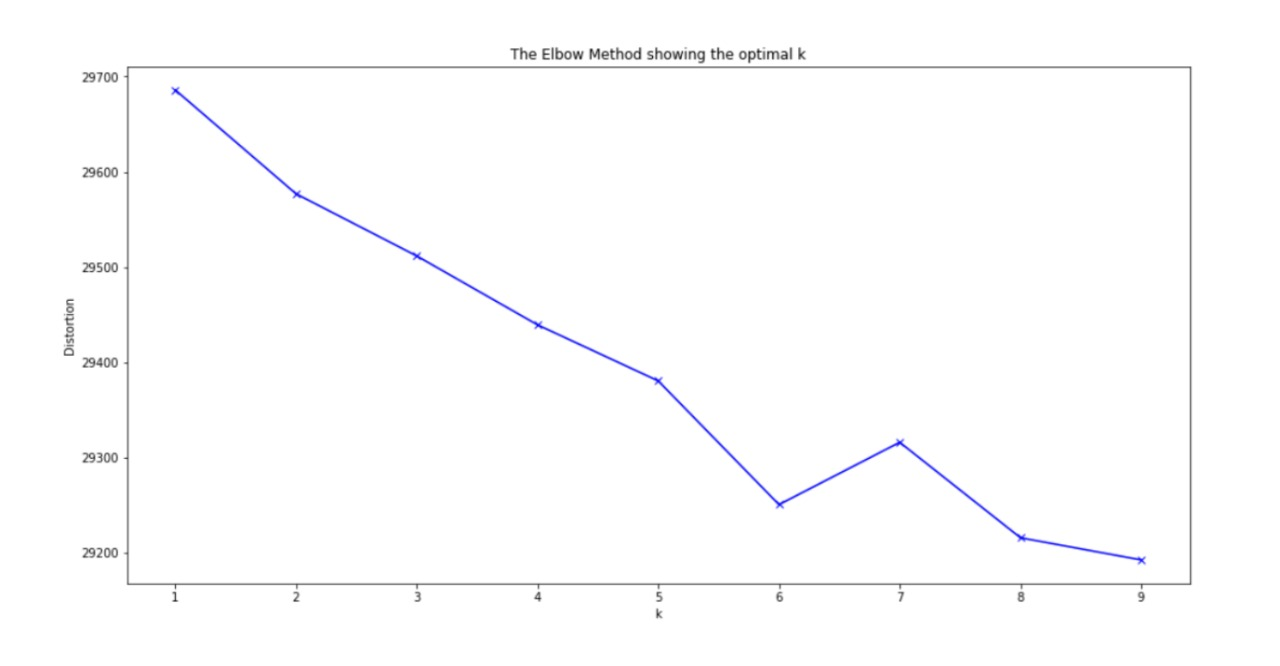
\includegraphics[width=1\linewidth, height=6cm]{images/elbow_method.jpg}
\caption{Elbow method}
\label{fig:elb}
\end{figure}

%------------------------------------------------

\section{Results}

From this graph it can be seen that 6 clusters are an optimal size. From here we are
able to view top-10 words from each cluster, thus those which are at the center of it
and represent a certain group of products. 


\begin{table}[h]
\centering
\caption{Clusters obtained}
\begin{tabular}{llllll}
\centering

CLuster 0 & Cluster 1 & Cluster 2 & Cluster 3 & Cluster 4 \\
\hline \hline 

\small body & golf & sports & bike & count   \\
\hline
\small oil & mens & football & bicycle & coffee   \\
\hline
\small organic & balls & soccer & cycling & protein   \\
\hline
\small butter & glove & basketball & road & tablets\\
\hline 
\small lotion & footjoy & tennis & mtb & roast \\
\hline
\end{tabular}
\end{table}


At the end a would like to reproduce the Schrödinger equation, just because I could not find any more formulas for this topic:

\begin{equation}
    i \hbar \frac{\partial}{\partial t} \Psi(x, t)=\left[-\frac{\hbar^{2}}{2 m} \frac{\partial^{2}}{\partial x^{2}}+V(x, t)\right] \Psi(x, t) \cite{berezin2012schrodinger}
\end{equation}


\clearpage

\bibliographystyle{plain}
\bibliography{bib.bib}

\end{document}
